In diesem Kapitel wird das erste Problem- bzw. Lernszenario vorgestellt. Ursprünglich war geplant, dem Titel dieser Arbeit folge zu leisten und ausschließlich das Ameisen-Agentenspiel (\glqq AntGame\grqq{}) zu behandelt. Ursprünglich ist dieses Beispiel mit dem Namen \glqq Jumping Dino\grqq{} entstanden, um die implementierten Algorithmen des RL bei einem scheinbar trivialeren Problem nachzuvollziehen.
\par 
Es stellte sich jedoch heraus, dass dieses episodiale Problem sehr gut geeignet ist, um das Konvergenzverhalten bei der Suche nach einer optimalen Strategie unter verschiedenen Bedingungen zu untersuchen. Vor allem eine Einschätzung darüber, welche Algorithmen (Monte-Carlo Methoden, \textit{SARSA}, \textit{Q-Learning}) für welche Problemszenarien praktikabel sind oder nicht, kann durch diese Untersuchung erlangt werden. 
\par 
Im nachfolgenden Unterkapitel wird zunächst die Problemstellung erläutert und die möglichen Modellierungen der Umwelt vorgestellt. Anschließend werden die Zustands- und Aktionsräume für die einzelnen Szenarien definiert, die dann als Grundlage für die Ergebnisse dienen, die in Kapitel 5 aufgeführt werden. Abgeschlossen wird dieses Kapitel mit der Modellierung einer passenden Belohnungsfunktion.

\subsubsection{Problemstellung}
Der Name \glqq Jumping Dino\grqq{} ist gewählt worden, weil das Beispiel an das bekannte Minigame \glqq T-Rex Runner\grqq{} von Google angelehnt ist, welches immer im Google Chrome Browser erscheint, wenn keine Internetverbindung vorhanden ist. Zusammengefast geht es darum, dass ein Dino im richtigen Moment über Hindernisse springen muss, die fortlaufend, von dem rechten Bildschirmrand aus, auf ihn zukommen.
\par 
Die gesamte Spielwelt ist 800px breit, wobei der Dino stehts 50px vom linken Bildrand entfernt ist. Hindernisse und der Dino selbst sind als Quadrate definiert, mit der Seitenlänge 60px respektive 50px. Die maximale Höhe eines Sprungs, also der Abstand zwischen dem Boden und der unteren Kante des Dinos, beträgt 150px. Jeden Tick werden die Positionen der Akteure um einen gewisse Pixelanzahl angepasst, welches zugleich als Geschwindigkeit angesehen werden kann. Der Dino hüpft in allen Szenarien um 20px pro Tick, die Geschwindigkeiten der Hindernisse kann jedoch je nach Szenario variieren.
\par 
Auf eine aufwendige Visualisierung des Spielgeschehens wurde verzichtet, der Dino wird lediglich als grünes Quadrat dargestellt, die Hindernisse als schwarzes Quadrat. Es ergibt sich folgende Umwelt:
\begin{figure}[H]
    \begin{center}
    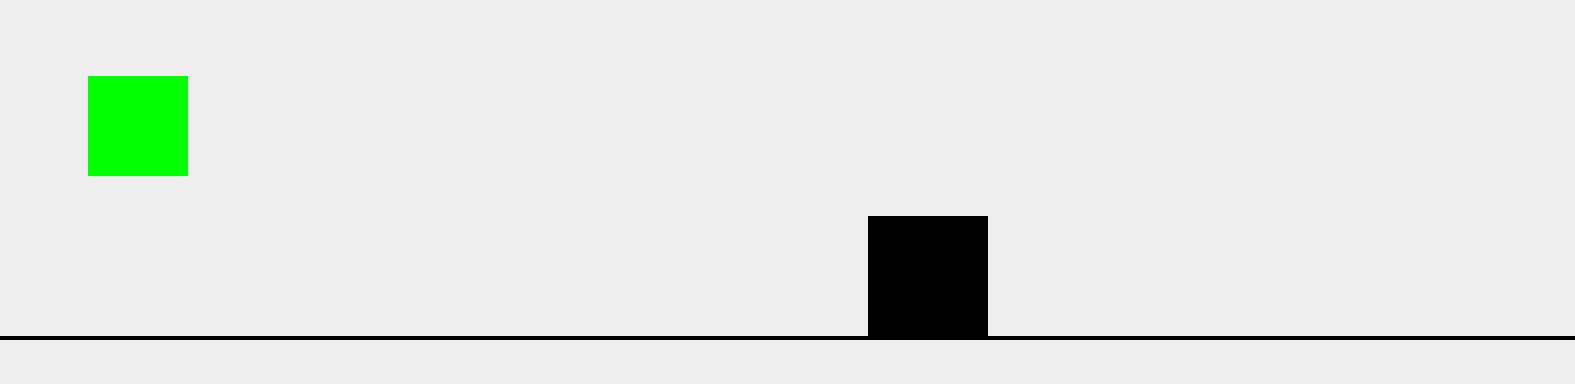
\includegraphics[width=0.5\textwidth]{images/jumpingDinoUmg.png}  \end{center}
    \caption{Jumping Dino Umgebung}
    \label{fig:2-Wege-2}
\end{figure}

Bei jedem Tick kann der Agent zwischen zwei Aktionen wählen, JUMP und NOTHING. Befindet sich der Agent bereits im Sprung, so ist es dennoch möglich die Aktion JUMP auszuwählen, sie hat jedoch keinen Effekt. Eine Episode endet, wenn eine Kollision zwischen dem Dino und dem Hindernis registriert wird.
\par 
Für die Untersuchungen wird zwischen zwei Szenarien unterschieden:
\par 
\textit{Simple}. Bei dieser Variante wandern die Hindernisse immer mit der gleichen Geschwindigkeit (30px pro Tick) nach links. Außerdem erscheinen sie immer im gleichen Abstand, d.h. erreicht die rechte Kante des Hindernisses den linken Bildschirmrand, so wird sofort ein neues Hindernis gespwant an der Position $x=860$. Es ergeben sich 31 mögliche Positionen, in der sich ein Hindernis in der Umwelt befinden kann ($x=860, x=830, \dots, x=-10, x=-40$).
\par 
\textit{Advanced}. Um die Umwelt anspruchsvoller zu gestalten, werden in diesem Szenario ein paar Änderungen vorgenommen. Statt einer festen Geschwindigkeit, bewegen sich die Hindernisse nun mit vier unterschiedlichen Geschwindigkeiten. Dies sorgt dafür, dass die Geschwindigkeit nun auch ein Faktor ist, der für einen Sprung des Dinos entscheidend ist. Bei sehr schnellen Hindernissen muss der Dino frühzeitig springen, um z.B. bei zwei aufeinanderfolgenden schnellen Hindernissen überhaupt in der Lage zu sein, das zweite Hindernis zu überspringen. Hingegeben muss er lernen, bei sehr langsamen Hindernissen erst sehr spät zu springen, um bei der Landung nicht zu kollidieren. Mit einer gleichen Wahrscheinlichkeit kann die Geschwindigkeit den Wert 10px, 21px, 48px oder 105px annehmen.
\par
Eine weitere Anpassung bei dem \textit{Jumping Dino Advanced} ist, dass die Hindernisse nicht immer mit dem gleichen Abstand spawnen, sondern ebenfalls zufällig mit vier unterschiedlichen Werten ($x=1630, x=1694, x=1718, x=1814$). Insgesamt ergeben sich 827 mögliche Positionen, die ein Hindernis einnehmen kann.

\subsubsection{Zustandsmodellierung}
Für eine korrekt gewählt Zustandsmodellierung, die genug aber nicht redundante Informationen beinhaltet, um die optimalen Entscheidung zu treffen, ist zunächst die Problemstellung genauer zu betrachten. 
\par 
In dem \textit{Jumping Dino Simple} Szenario muss der Agent lernen, im richtigen Moment die Aktion JUMPING durchzuführen. Anders ausgedrückt, kann der Agent in der Theorie immer die Aktion NOTHING wählen, muss aber bei einem bestimmten Abstand zu dem Hindernis die Aktion JUMP ausführen. Im Grunde ist dies eine Schwellwertsuche, bei der vorerst angenommen wird, dass alleine die Distanz zu dem Hindernis ausreichend ist, um das Problem zu lösen.
\par 
Den Zustand nur anhand der Distanz zu verwirklichen ist bei der \textit{Advanced} Variante nicht ausreichend, um optimale Entscheidung zu treffen. Schnelle Hindernisse müssen frühzeitiger übersprungen werden, langsame hingehen erst kurz vor einer Kollision. Eine zweite Information muss somit gegeben sein, die Geschwindigkeit der Hindernisse.
\par 
Im späteren Verlauf der Untersuchungen zu dem Konvergenzverhalten, die in Kapitel 5 näher erläutert werden, stellt sich heraus, dass der Zustand um eine boolische Flag erweitert werden muss, die aussagt, ob der Dino sich im Sprung befindet oder nicht. 
Es ergeben sich insgesamt drei unterschiedliche Zustandsmodellierungen, die auf folgenden Variablen beruhen:
\begin{itemize}
 \item $dist$: \textit{Integer}, Abstand zwischen rechter Kante des Dinos und  linker Kante des Hindernisses
 \item $inJump$: \textit{Boolean}, Boolischer Wert, ob sich der Dino in einem Sprung befindet und somit die Aktion \textit{JUMP} keine Auswirkung hat.
 \item $obsSpeed$: \textit{Integer}, Geschwindigkeit, mit der das Hindernis nach links wandert. Bei dem \textit{Jumping Dino Advanced} kann diese Variable vier unterschiedliche Werte annehmen.    
\end{itemize}
\begin{equation}
    Z_{1} =  \begin{bmatrix} dist\\   \end{bmatrix}, \quad
    Z_{2} =  \begin{bmatrix} dist \\ inJump   \end{bmatrix}, \quad
    Z_{3} =  \begin{bmatrix} dist \\ inJump \\ obsSpeed   \end{bmatrix}
\end{equation}

Die Kombination des Zustandraumes mit den zwei ausführbaren Aktionen ergibt die Anzahl der möglichen Zustands-Aktions-Paare, für die Werte in der Aktions-Nutzentabelle gespeichert werden. Es gibt zwei Szenarien \textit{Simple} und \textit{Advanced} und drei Zustandsmodellierungen $Z_1, Z_2$ und $Z_3$.
Für das Szenario \textit{Simple} ist die Modellierung $Z_3$ redundant, da die Variable $obsSpeed$ nur einen Wert annehmen kann. Wie bereits erwähnt, muss der $obsSpeed$ bei der \textit{Advanced} Variante gegegen sein. 
\par 
Wichtig zu erwähnen ist, dass diese Werte sich auf die tatsächlich möglichen $(s,a)$-Paare beziehen. D.h. für die \textit{Simple} Variante ergeben sich für $Z_2$ in der Theorie 62 mögliche Zustände (Abstand des Hindernisses * im Sprung oder nicht, $31*2$). Die Nutzentablle registriert jedoch nur 58 Zustände, da einige Zustände gar nicht erreicht werden können. Für die Abstände $-40, -10, 20$ und $50$ existieren nur die Kombinationen mit $inJump = true$. Der Dino musste vorher springen bzw. befindet sich im Sprung, da ansonsten die Episode zuvor bei einer Kollision vorzeitig beendet werden würde. Das erklärt die abweichenden Größen im Vergleich zu den Werten der theoretischen Kombinationen.
\par 
Gesamtanzahl aller gespeicherten Aktions-Nutzen:
\begin{equation}
G_{simple, Z_1} = 62, \quad
G_{simple, Z_2} = 116, \quad
G_{advanced, Z_3} = 4146 \quad 
\end{equation}


\subsubsection{Belohnungsfunktion}
Im Kapitel \ref{sec:belohnung} wurde darauf eingegangen, wie in eine Belohnungsfunktion gewählt werden sollte. Die Schlussfolgerung war, dass eine Belohnungsfunktion dem Agenten vermitteln soll, \textit{was} er erreichen soll und nicht \textit{wie} er es erreichen soll \cite[S.~54]{Sutton1998}.
\par 
Die Aufgabe des hüpfenden Dinos besteht darin, die Episode so lang wie möglich zu überleben. Anders formuliert soll die Episode eine maximale Anzahl von Zeitstempeln andauern. Um dieses Ziel als Belohungssignal zu modellieren, reicht es aus dem Agenten zu jedem Zeitpunkt $t$ eine Belohnung von +1 mitzuteilen. Einzige Ausnahme ist hierbei das Erreichen eines Terminalzustandes. Kollidiert der Dino mit einem Hindernis, so erhält er die Belohnung +0 und die Episode ist beendet. Der Gewinn einer Episode richtet sich somit nach der Anzahl der Zeitstempel. Eine explizite Modellierung der Hindernisse oder die Vergabe von Belohnungen für das Überspringen dieser ist nicht notwendig, da der Agent implizit lernt, Hindernisse zu überspringen, um die Summe der Belohnungen zu maximieren. 
\par 
//TODO
\par 
